\begin{frame}{Tools to improve traffic indicators}
    \begin{columns}
    \begin{column}{0.5\textwidth}
    \only<1-2>{
    \begin{exampleblock}{Optimization}
    In order to optimize the \emph{cost} $f(x)$, the value of $x$ should be found, while respecting the constraints
        \begin{equation*}
        x^*=
        \begin{aligned}
        &\underset{x}{\min}& &f(x)\\
        &\text{s.t}& &x\geq0.5
        \end{aligned}
        \end{equation*}
    \end{exampleblock}
    }
    \only<3->{
    \begin{exampleblock}{Design \& Constraints}  
    \begin{itemize}[<+->]
        \item Duty cycle $\bar{u}$ as control variable
        \item Maximize network throughput + minimize the balance
        \item Model-based predictions computed by using the Avg-CTM
    \end{itemize}
    \end{exampleblock}
    }
    \end{column}
    \begin{column}{0.5\textwidth}
    \begin{figure}
    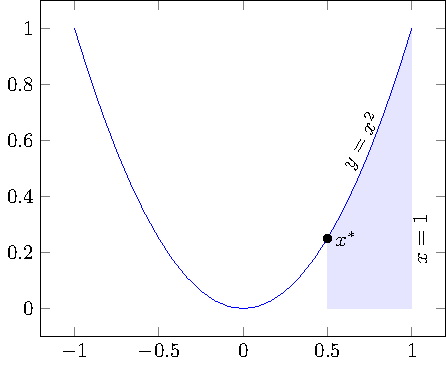
\includegraphics[width=\textwidth]{fig_65_square}
    \end{figure}
    \onslide<2->{
    \begin{exampleblock}{Optimal criteria}
        \[
            \underset{\bar{u}}{\min}\ Bal\left(\bar{u}(t)\right) - TTD\left(\bar{u}(t)\right) + R\left(\bar{u}(t,T)\right)
        \]        
    \end{exampleblock}
    }    
    \end{column}
    \end{columns}


\end{frame}